\section{Background}

\begin{itemize}
\item Blockchain
\item Proof of Stake
\item Transactions and Transaction costs
\item Ethereum and Smart Contracts
\item Hashing basics?
\end{itemize}

\subsection{Blockchain}

A new concept for trustless, decentralized and transparent information processing and storage has been developed, introduced and already integrated into several mainstream applications in the last years. Bitcoin, developed by an unknown person or group under the name of Satoshi Nakamoto, led this initiative back in 2008 with its open-source, peer-to-peer network which cryptographically stores records in a chain and serves as a distributed ledger, this was named the Blockchain. The currency in which these operations were valued and paid for with was called Bitcoin, and it was the first decentralized digital currency.
Blockchains are essentially continuously growing lists of information which are linked together and secured using cryptography. The main benefit of Blockchains is that they are designed to be incorruptible, and that the data they hold cannot be unintentionally modified since the entire history of the chain is always stored and recorded on it. It is verified by peers and transparent to each user.
Blockchain technology is a mixture of various computing and economic concepts especially in financial sectors, including peer-to-peer systems, cryptography based, consensus protocols, decentralized storage, decentralized processing and smart contracts. The consolidation of these concepts makes blockchains as another innovation and as a programmable platform and system at the same time. Blockchains consist of specific properties including immutability and transparency of cryptographically-secured and peer-recorded transactions, which have been settled upon by consensus on the network. Being able to build up trustless interactions and business disintermediation continues to be one of the most important objectives of using blockchains.

\subsection{Smart Contracts}
Computer programs that are executed automatically when conditions (terms) of the contract have been met. Understanding smart contracts in a high-level aspect are the same as standard contracts. While a standard contract enforces the terms of a contract (regularly by law), a smart contract actualizes this enforcement of terms through network consensus and online cryptography secure systems. These programs are executed in a trustless and carefully designed way in the network and are referred as Smart Contracts. Ethereum is one of the most known platforms, it empowers developers to create their own smart contracts and creating decentralized applications in the blockchain [\cite{Buterin2014}]. Upon creation of smart contracts, they need to be executed in a secured runtime environment. Therefore, an Ethereum Foundation team project developed the Ethereum Virtual Machine (EVM) which is the runtime enviroment for Smart Contracts. Putting it in simpler understanding, EVM is a virtual machine that continues running on every node in the network and executes smart contracts. In addition, it is isolated that no framework or filesystem access is possible, thus, to ensure determinism. One vital part of the way the EVM works is that each and every task that is executed inside the EVM, is executed by each full node. This is a crucial part of the Ethereum 1.0 consensus model and has the advantage that any contract on the EVM can call some other contract at zero cost, however, it also has its disadvantages that the computational steps on the EVM are exceptionally costly [\cite{Buterin2014}]. In order that the Ethereum network is not being abused or being deliberately attacked, the Ethereum protocol charges a fee for every computational step. The way this cost is paid in Ethereum blockchain i’s through the attribute called gas. The fee or the price of the gas is deteremined on market-basis; meaning it is decided by the economic concept of market where supply meets demand among users and miners' willingness to mine the next block in the network (blockchain). Furthermore, understanding the way how fees work, is that every transaction alongside other attributes must contain the 'gasPrice', which is the fee that the transaction pays per unit of gas, and 'startGas' being the maximum amount of unit of gas that you are willing to pay for a transaction. Therefore, at every execution of transaction a prior evaluation of a transaction cost is done [\cite{Buterin2014}].
				\[ gasCost(Tx)= {gasPrice *  startGas}\]
To understand to which extent the usage of the EVM makes sense, it can mainly incorporate running business logic applications ("if this then that"), confirming signatures and other cryptographic objects [\cite{Ethereum2017}. On the other hand, any utilization which incorporates using EVM as a file storage, platform or anything to do with GUI, it does not fit under the reasonable use due to its tremendous costs. Therefore, usage of on-chain code execution with today's blockchain implementations, implies furthest to be at the stage of doing simple programming functions. Nevertheless, in order to be able to use Smart Contracts, higher level programming languages which compile EVM code have been developed such as Solidity, Serpent, LLL.



\begin{figure}[h]
\centering
\includegraphics[width=0.4\textwidth]{images/smartcontracts.png}
\caption{\label{fig:Smartcontracts}www.blockgeeks.com}
\end{figure}




\subsection{Blockchain-level Protocol: UTXO and Account Model}

The need of secure of value transfer lead to invention of building tamper-resistant systems. The way how transactions are handled, is one of the main characteristics of the blockchain technology. They are the smallest building pieces of a blockchain system. Transaction level consensus are exceptionally expensive, therefore, are bundled together forming a block or a unite of consensus. With every block creation chained to the previous block (through previous block hash) in the network forming chains of blocks, therefore, creating the blockchain.


\begin{figure}[h]
\centering
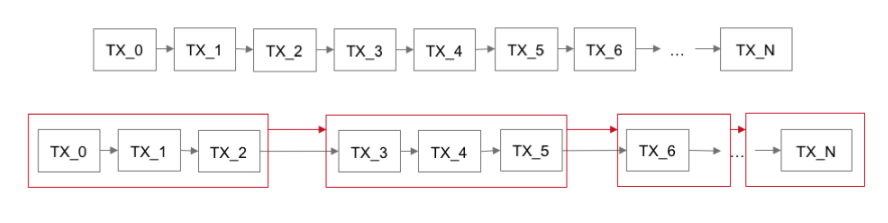
\includegraphics[width=0.8\textwidth]{images/transactions_blocks.png}
\caption{\label{fig:Transactions}Transactions order bundeled into blocks.}
\end{figure}


With blockchain being a mutual, decentralized, distributed state machine, this implies that all nodes (users of the blockchain framework) freely hold their own particular duplicate of the blockchain, and the current known "state" is calculated by handling every transaction in order as they show up in the blockchain. The way how each transactions and blocks are mined (processed) in the network differ from implementation. With the introduction of Bitcoin’s Unspent Transaction Output (UTXO) and later Ethereum project with its concept of Account Model state model. Further in this report we provide an explanation of each state models, purpose and use cases.

\subparagraph{Unspent Transaction Output (UTXO)}

With Bitcoin being a transaction-centric state model UTXO model; which specifies who is allowed to use the output of the transaction moves the estimation of some bitcoin from one address to other address. A transaction changes the state of the agreed-correct blockchain.

\begin{figure}[h]
\centering
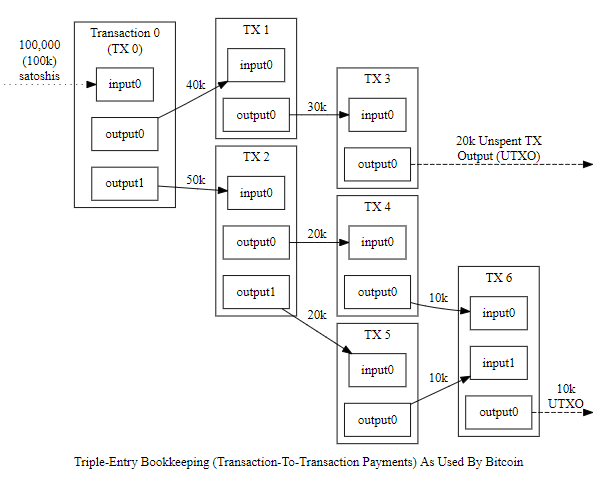
\includegraphics[width=0.8\textwidth]{images/UTXO.png}
\caption{\label{fig:UTXO}UTXO Transactions example}
\end{figure}

Understanding the above example of how Bitcoin transactions work which are UTXO model, transactions contain one or more input and output vice versa. An input is a reference to an output from the previous transaction. Whereas an output specifies the amount and an address. With the input pointing always referencing from a previous transaction, provides and uninterrupted stream of value amongst addresses

\subparagraph{UTXO Transaction Validation}
\begin{itemize}
\item Guarantees inputs have not yet been spent
\item Checking if the signatures match with addresses of transactions inputs
\item Total of output values is equivalent to total of input values
\end{itemize}


\subparagraph{Benefits of UTXO Model:}
\begin{itemize}
\item \textbf{Higher level of privacy:} if a user uses another address for every transaction that they receive then it will quite hard to find the correlation of accounts to each other. This model suits greatly for currency use, however significantly less to subjective decentralized applications (DApp), since DApps frequently include monitoring complex packaged state of users which becomes difficult to be achieved.
\item \textbf{Potential scalability paradigms:} UTXOs are more hypothetically compatible with certain types of scalability paradigms.
\end{itemize}

\subparagraph{Account Model}

Ethereum transactions, rather, utilize an architecture depending on global state storage of accounts, balances, code, and storage. The balances of accounts are kept as global state. Moreover, the having the value distribution of a state-centric meaning of transaction specifies sender and the receiver account and its not referenced to the previous transactions. Transaction include binary data (its payload) and Ether

\begin{figure}[h]
\centering
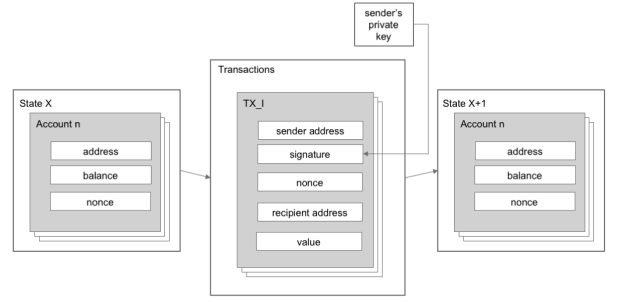
\includegraphics[width=1.0\textwidth]{images/account_model.png}
\caption{\label{fig:account model}Ethereum Blockchain Account Model Transactions}
\end{figure}


\subparagraph{Account Model Transaction Validation}
\begin{itemize}
\item Check whether signatures match with address of the sender
\item Ensuring that the current nonce matches the nonce from the sender’s account. If that’s the case, it automatically increments the nonce of the sender
\item Guarantee the sender's balance is bigger or equal with than the transaction value
\end{itemize}

\subparagraph{Benefits of Account Model:}
\begin{itemize}
\item \textbf{Huge space savings:}Due to the fact that each transaction only needs to create one reference, one signature and one output
\item \textbf{Simplicity:} Light clients are able to access the whole records related to an account through scanning down the state tree in a specific direction.
\end{itemize}


\section{Integrity Checks}
\sectionnames{Simon Fallnich}

	This section describes basic principles to verify the integrity of data from an untrusted source.

	% Hashing
	\subsection{Hashing}
	\label{subsec:hashing}

		A \emph{hash function} maps an input of arbitrary length to an ouput of fixed length, referred to as \emph{hash} \cite{menezes1996}.
		Although hash functions are used for a wide range of applications in the domain of computer science, the class of \emph{cryptographic hash functions} is primarily relevant for our application.
		A cryptographic hash function, or \emph{one-way function}, is a hash function which is infeasible to invert.
		This essential property lays the foundation for efficient integrity check mechanisms as the resulting hashes can be used to securely proof equality of the underlying data.

	% Merkle Tree
	\subsection{Merkle Tree}
	\label{subsec:merkle-tree}

		\begin{figure}
			\centering
				\begin{tikzpicture}[line cap=round, line join=round, yscale=0.8]
					% First layer
					\node [circle, draw=black, fill=white, minimum size = 1cm] (node-1-1) at (0, 0) {$H_0$};
					% Second layer
					\foreach \a [count=\x] in {1, 2}
						\node [circle, draw=black, fill=white, minimum size=1cm] (node-2-\x) at (-12 + 8 * \x, -2) {$H_\a$};
					% Third layer
					\foreach \a [count=\x] in {3, ..., 6}
					  \node [circle, draw=black, fill=white, minimum size=1cm] (node-3-\x) at (-10 + 4 * \x, -4) {$H_\a$};
					% Fourth layer
					\foreach \a [count=\x] in {7, 8}
					  \node [circle, draw=black, fill=white, minimum size=1cm] (node-4-\x) at (-9 + 2 * \x, -6) {$H_\a$};
					% First data layer
					\foreach \a [count=\x] in {0, ..., 2}
					  \node [draw=gray, text=gray, fill=white, minimum size=0.8cm] (data-1-\x) at (-6 + 4 * \x, -6) {$D_\a$};
					% Second data layer
					\foreach \a [count=\x] in {3, 4}
					  \node [draw=gray, text=gray, fill=white, minimum size=0.8cm] (data-2-\x) at (-9 + 2 * \x, -8) {$D_\a$};
					% First layer arrows
					\foreach \a in {1, 2}
					  \draw (node-1-1) -- (node-2-\a);
					% Second layer arrows
					\foreach \a in {1, 2}
					  \draw (node-2-1) -- (node-3-\a);
					\foreach \a in {3, 4}
					  \draw (node-2-2) -- (node-3-\a);
					% Third layer arrows
					\foreach \a in {1, 2}
					  \draw (node-3-1) -- (node-4-\a);
					\draw [draw=gray] (node-3-2) -- (data-1-1);
					\draw [draw=gray] (node-3-3) -- (data-1-2);
					\draw [draw=gray] (node-3-4) -- (data-1-3);
					\draw [draw=gray] (node-4-1) -- (data-2-1);
					\draw [draw=gray] (node-4-2) -- (data-2-2);
				\end{tikzpicture}
			\caption{A binary Merkle tree with five leaf nodes. While $H_i$ denotes the hash which is stored for the node with index $i$, $D_j$ denotes the data block with index $j$.}
			\label{fig:merkle-tree}
		\end{figure}

		\begin{figure}
			\centering
				\begin{tikzpicture}[line cap=round, line join=round, yscale=0.8]
					% First layer
					\node [circle, draw=black, fill=white, minimum size = 1cm] (node-1-1) at (0, 0) {$H_0^r$};
					% Second layer
					\node [circle, draw=black, fill=white, minimum size=1cm] (node-2-1) at (-4, -2) {$H_1^r$};
					\node [circle, draw=black, fill=white, minimum size=1cm] (node-2-2) at (4, -2) {$H_2^s$};
					% Third layer
					\node [circle, draw=black, fill=white, minimum size=1cm] (node-3-1) at (-6, -4) {$H_3^r$};
					\node [circle, draw=black, fill=white, minimum size=1cm] (node-3-2) at (-2, -4) {$H_4^s$};
					% Fourth layer
					\node [circle, draw=black, fill=white, minimum size=1cm] (node-4-1) at (-7, -6) {$H_7^s$};
					\node [circle, draw=black, fill=white, minimum size=1cm] (node-4-2) at (-5, -6) {$H_8^r$};
					% Second data layer
					\node [draw=gray, text=gray, fill=white, minimum size=0.8cm] (data-2-2) at (-5, -8) {$D_4^s$};
					% First layer arrows
					\foreach \a in {1, 2}
					  \draw (node-1-1) -- (node-2-\a);
					% Second layer arrows
					\foreach \a in {1, 2}
					  \draw (node-2-1) -- (node-3-\a);
					% Third layer arrows
					\foreach \a in {1, 2}
					  \draw (node-3-1) -- (node-4-\a);
					\draw [draw=gray] (node-4-2) -- (data-2-2);
				\end{tikzpicture}
			\caption{An exemplary Merkle tree integrity check. A superscript $s$ denotes that the respective value is given by the untrusted sender, whereas a superscript $r$ denotes a value which is computed by the receiver.}
			\label{fig:merkle-tree-proof}
		\end{figure}

		A \emph{Merkle} tree, or \emph{hash tree}, is a tree in which every leaf node stores the hash of a data block and every non-leaf node stores the hash of the concatenated hashes of its children \cite{merkle1987}.
		This structure enables efficient, partial integrity checks on large data sets.
			
		\autoref{fig:merkle-tree} shows a binary Merkle tree with five leaves.
		As the node with index $4$ is a leaf, the stored hash $H_4$ can be computed as
		\begin{equation}
			H_4 = h(D_0),
		\end{equation}
		where $h(\cdot)$ is the employed hash function and $D_0$ is the corresponding data block for this particular leaf node.
		In contrast, the node with index $3$ is a non-leaf node and its hash $H_3$ can hence be calculated as
		\begin{equation}
			H_3 = h(H_7 + H_8),
		\end{equation}
		where $H_7 + H_8$ denotes the concatenation of the hashes of nodes $7$ and $8$.
		Similarly, the hash of the root node $H_0$, also referred to as \emph{root hash} or \emph{Merkle root}, results as
		\begin{align}
			H_0 &= h(H_1 + H_2)\\
			&= h(h(H_3 + H_4) + h(H_5 + H_6))\\
			&= h(h(h(H_7 + H_8) + h(D_0)) + h(h(D_1) + h(D_2)))\\
			&= h(h(h(h(D_3) + h(D_4)) + h(D_0)) + h(h(D_1) + h(D_2))).\label{eq:merkle-recursive}
		\end{align}

		\autoref{eq:merkle-recursive} indicates that, due to the recursive nature of the hash computation, there is no possibility of altering any data block without changing the root hash as well.
		Therefore, it is sufficient to know the root hash in order to be able to verify the integrity of any data block in the tree.

		For instance, a sender wants to send data block $D_4$ to a receiver, which only knows the root hash $H_0$.
		Let $D_4^s$ denote the sent data block, where the superscript $s$ indicates that this data comes from the untrusted sender and could be different from the original $D_4$.
		In addition to the possibly altered data block $D_4^s$, the sender sends the hashes $H_2^s$, $H_4^s$ and $H_7^s$.
		With the given data block and the given hashes, the sender then resconstructs the corresponding Merkle tree to compute the root hash $H_0^r$ (see \autoref{fig:merkle-tree-proof}), where the superscript $r$ indicates that a hash is computed by the receiver:
		\begin{align}
			H_8^r &= h(D_4^s)\\
			H_3^r &= h(H_7^s + H_8^r)\\
			H_1^r &= h(H_3^r + H_4^s)\\
			H_0^r &= h(H_1^r + H_2^s).
		\end{align}
		If the computed root hash $H_0^r$ equals the known root hash $H_0$, the sender has successfully verified the integrity of the given data block ($D_4^s = D_4$) without knowing any other data block or non-root hash beforehand.
		This holds since, with the use of a cryptographic hash function (see \autoref{subsec:hashing}), the sender cannot determine a hash $H_7^\prime$ which, combined with an altered data block $D_4^\prime$, would yield the correct parent hash $H_3$.\footnote{For this, the sender would have to solve $H_3 = h(H_7^\prime + D_4^\prime)$ for $H_7^\prime$, which requires the infeasible inversion of the cryptographic hash function $h(\cdot)$.
		One might argue that the hash $H_3^r$ does not need to equal $H_3$ as long as the resulting root hash $H_0^r$ equals $H_0$ --- but this just propagates the problem of solving for an unknown input to $h(\cdot)$ to another level in the tree.}


\subsection{The Concept of Query Completeness}
The possibility to query RDBMS is a pivotal functionality of those systems and thus represents a great entry point for efforts to link the technologies of blockchain and RDBMS as targeted in this project. The trust that today’s users of RDBMS put into the correctness of the returned results for their queries could be nullified by the trustlessness offered by the blockchain - trustless query results in a sense. Right now, no user can be sure if her results were not tampered with or only part of the truth was returned to her.
Through an initial slide set from our supervisor Jacob Eberhardt we were introduced to the concept of query completeness which aims at achieving completely trustless queries. The general idea is to use the blockchain and its properties to counteract the four ways a database system could falsify the query results. In detail, the following measurements have to be prevented:
The database system could try to not consider all database records while performing the query. This means, a mechanism has to be implemented that verifies that all records were looked at.
The database system could try to add records to the query results that were not part of the database before. To counteract, a trustless systems needs to show that all considered records were part of the database already and that the returned results are actual database entries.
The database system could try to leave out actual database records that fulfill the query in the returned set of records. Accordingly, we need to proof that that all records that fulfill a user’s query find their way into the results that the user obtains.
The database system could try to include actual database records that do not fulfill the query in the returned set of records. A trustless system thus has to check that only records that fulfill the query are returned to the user.
Any system that successfully counteracts these ways to counterfeit query results achieves query completeness as defined here.
